\subsection{Foundations of Quality in IT}

\subsubsection{Quality in IT}

\indent

\noindent\textbf{Quality in IT} refers to how well a software product or IT service meets stakeholder needs and expectations, while being reliable, secure, and maintainable.

\bigskip

\noindent Dimensions of Quality in Software:

\begin{itemize}
    \item Functionality: Does the system do what it’s supposed to do?
    \item Reliability: Can it perform consistently under expected conditions?
    \item Usability: Is it user-friendly and accessible?
    \item Efficiency: Does it use resources (CPU, memory, bandwidth) optimally?
    \item Maintainability: How easy is it to update, fix, or improve?
    \item Portability: Can it be deployed in different environments easily?
    \item Security: Can it protect data and resist threats?
\end{itemize}

\bigskip

\noindent Why does Quality matter in IT?

\begin{itemize}
    \item \textbf{Business perspective}: Enhances customer satisfaction, reduces costs of rework, builds trust.
    \item \textbf{Technical perspective}: Prevents bugs, system crashes, and vulnerabilities.
    \item \textbf{Professional/ethical perspective}: IT professionals have a responsibility to deliver safe and reliable systems.
\end{itemize}

\bigskip 

\noindent Cost of Poor Quality in IT

\begin{itemize}
    \item Direct costs: Bug fixes, downtime, data loss.
    \item Indirect costs: Reputational damage, loss of clients, potential legal issues.
\end{itemize}

\subsubsection{Quality Assurance}

\indent 

\textbf{Quality Assurance (QA)}: A \textbf{proactive}, \textbf{process-oriented approach} that ensures software and IT services meet defined standards and stakeholder expectations.

Focuses on \textbf{preventing defects} rather than just detecting them. Ensures that the \textbf{processes used to create deliverables} are effective and reliable.

\bigskip

\noindent Objectives:

\begin{itemize}
    \item Ensure that software meets requirements and complies with standards.
    \item Minimize defects by improving development and testing processes.
    \item Improve efficiency of teams through standardized workflows.
    \item Build customer confidence and trust in IT systems.
\end{itemize}

\subsubsection{Quality Control}

\indent 

\textbf{Quality Control (QC)}: A reactive, product-oriented process that ensures deliverables meet defined quality standards.

Focuses on \textbf{detecting defects} in the product or service after development has begun. Ensures the output matches requirements and specifications.

\bigskip

\noindent Objectives:

\begin{itemize}
    \item Verify that the final product is reliable and fit for purpose.
    \item Detect and document defects or deviations from requirements.
    \item Ensure compliance with customer and regulatory standards.
    \item Provide feedback for process improvement (links back to QA).
\end{itemize}

\subsubsection{Testing}

\indent 

\textbf{Software Testing}: The process of \textbf{executing a system or application} with the intent of finding defects and verifying it meets specified requirements.

A \textbf{subset of Quality Control (QC)}.

Focused on \textbf{validation} (Are we building the right product?) and \textbf{verification} (Are we building the product right?).

\bigskip

Main purpose of testing:

\begin{itemize}
    \item To find defects before the software reaches users.
    \item To ensure the product meets functional and non-functional requirements.
    \item To reduce risks (financial, safety, reputational).
    \item To increase confidence in the product.
\end{itemize}

\subsection{Quality Assurance in IT}

\indent 

\noindent\textbf{Quality Assurance (QA) in IT}: A systematic process to ensure that IT systems, software, and services \textbf{consistently meet requirements}, \textbf{industry standards}, and \textbf{user expectations}.

\bigskip

It goes beyond software, it covers: \textbf{Infrastructure} (servers, networks, cloud), \textbf{Processes} (SDLC, ITIL practices), \textbf{Information Security} (compliance, audits).

\subsubsection{QA standards}

\indent 

\noindent\textbf{Quality Standards}: Agreed-upon criteria, guidelines, or frameworks used to \textbf{ensure IT systems, software, and processes meet quality requirements}.

\bigskip

They provide \textbf{consistency, reliability, and assurance} across projects, teams, and organizations.

Standards are often \textbf{internationally recognized} (ISO, IEEE) or \textbf{industry specific}.

Quality standards are important as:

\begin{itemize}
    \item Ensures processes are repeatable and auditable.
    \item Provides benchmarks for performance, security, and reliability.
    \item Supports compliance with laws and regulations.
    \item Reduces risk of failures and costly defects.
    \item Facilitates continuous improvement and professional accountability.
\end{itemize}

\subsubsection{ISO 9000}

\indent

\textbf{ISO 9000} is a family of international standards developed by the \textbf{International Organization for Standardization (ISO)}.

Goal: Ensure organizations consistently deliver \textbf{products} and \textbf{services} that \textbf{meet customer and regulatory requirements}.

\bigskip

\noindent Main principles:

\begin{itemize}
    \item Customer focus: Meeting or exceeding customer expectations.
    \item Leadership: Establishing unity of purpose and direction.
    \item Engagement of people: Involving staff at all levels.
    \item Process approach: Managing activities as processes for efficiency.
    \item Improvement: Continuous organizational learning and enhancement.
    \item Evidence-based decision making: Using data and facts for decisions.
    \item Relationship management: Managing relationships with stakeholders (suppliers, partners, regulators).
\end{itemize}

\bigskip

\noindent Why is ISO-9000 important in IT?

IT projects often involve complex processes, multiple stakeholders, and high risks.

ISO 9000 ensures:

\begin{itemize}
    \item Clear processes for software development, testing, and delivery.
    \item Consistency across multiple projects and teams.
    \item Customer trust in reliable and repeatable outcomes.
    \item Continuous improvement in IT service delivery
\end{itemize}

\bigskip

\noindent Benefits of ISO-9000

\begin{itemize}
    \item Standardized documentation and reporting.
    \item Better process control and efficiency.
    \item Fewer defects and failures.
\end{itemize}

\subsubsection{ISO 27001}

\indent

\textbf{ISO/IEC 27001} is an international standard for \textbf{Information Security Management Systems (ISMS)}.

Published by the \textbf{International Organization for Standardization (ISO)} and the \textbf{International Electrotechnical Commission (IEC)}.

Provides a \textbf{systematic approach} to managing sensitive company and customer information so it remains \textbf{confidential, accurate, and available}.

\bigskip

\noindent The main objectives of ISO27001 are:

\begin{itemize}
    \item Protect confidentiality, integrity, and availability (CIA triad) of information.
    \item Establish an ISMS: a structured framework of policies, processes, and controls.
    \item Reduce risks such as data breaches, hacking, insider threats, or human errors.
    \item Provide compliance with legal, regulatory, and contractual requirements.
\end{itemize}

\bigskip

\noindent The key components of ISO 27001 are:

\begin{itemize}
    \item \textbf{Risk Assessment}: Identify and evaluate information security risks.
    \item \textbf{Security Controls}: 114 controls grouped into 14 categories
    \item \textbf{Continuous Improvement}: Regularly monitor, review, and improve the ISMS.
    \item \textbf{Management Involvement}: Top management commitment is essential.
\end{itemize}

\bigskip

ISO 27001 is important in IT as:

\begin{itemize}
    \item IT systems handle sensitive data: customer records, financial data, intellectual property and Cyber threats are increasingly sophisticated.
    \item ISO 27001 helps organisations:
    \begin{itemize}
        \item Demonstrate trustworthiness to clients.
        \item Reduce the likelihood and impact of breaches.
        \item Align with other compliance requirements (e.g., GDPR, HIPAA, APRA in Australia).
    \end{itemize}
\end{itemize}

\subsubsection{Quality Assurance and Governance Frameworks}

\indent 

A \textbf{governance framework} defines the structures, processes, and practices that ensure IT activities are aligned with \textbf{business objectives}, \textbf{regulations}, and \textbf{quality standards}.

\bigskip 

In QA, governance ensures that:

\begin{itemize}
    \item Quality processes are not ad-hoc but institutionalized.
    \item Roles and responsibilities are clearly defined.
    \item Compliance with standards (ISO, CMMI, IEEE, ITIL, etc.) is monitored.
\end{itemize}

\bigskip

\textbf{QA} ensures that products and processes meet agreed quality standards.

Governance provides the \textbf{oversight and accountability} to ensure QA is applied consistently across projects.

Together, they create a \textbf{culture of quality and accountability} in IT organizations.

\subsubsection{Key QA and Governance Frameworks}

\indent 

\begin{itemize}
    \item ITIL
    \begin{itemize}
        \item Focus: IT Service Management (ITSM).
        \item QA Role: Provides processes for incident, change, and problem management, ensuring consistent service delivery.
    \end{itemize}
    \item COBIT
    \begin{itemize}
        \item Focus: IT governance and management.
        \item QA Role: Emphasizes control, risk management, and process maturity.
    \end{itemize}
    \item CMMI
    \begin{itemize}
        \item Focus: Process maturity in software and systems engineering.
        \item QA Role: Provides a structured roadmap to process improvement across maturity levels.
    \end{itemize}
\end{itemize}

\subsubsection{The Deming Cycle}

\indent 

Also known as the \textbf{PDCA Cycle}: Plan $\xrightarrow{}$ Do $\xrightarrow{}$ Check $\xrightarrow{}$ Act.

A continuous improvement model used in quality assurance, process management, and governance frameworks.

This 4 stages are:

\begin{itemize}
    \item \textbf{Plan}: Identify problems or opportunities.
    \item \textbf{Do}: Implement the plan on a small scale.
    \item \textbf{Check}: Monitor and evaluate results against expected outcomes.
    \item \textbf{Act}: Standardize successful practices.
\end{itemize}

\subsubsection{Capability Maturity Model Integration (CMMI)}

\begin{figure}[h]
    \centering
    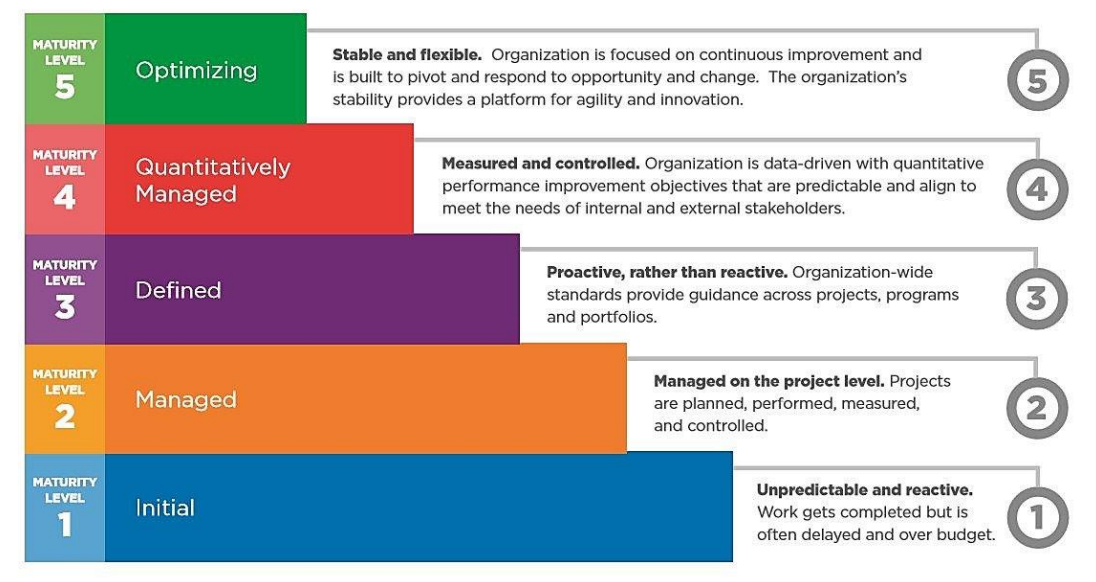
\includegraphics[width=0.9\linewidth]{figures/Week 8/CMMI.png}
\end{figure}

A \textbf{process improvement framework} that helps organizations \textbf{develop}, \textbf{refine}, and \textbf{measure maturity in processes} for software, systems, and service delivery.

Used in IT, engineering, defense, healthcare, and finance industries.

CMMI integrates closely with QA because QA ensures \textbf{processes are followed consistently}, CMMI ensures those processes are \textbf{mature, measurable, and improving}.

Often combined with \textbf{ISO 9001} and the \textbf{Deming Cycle} for continuous process improvement.

\subsubsection{The Deming cycle and CMMI Maturity Levels}

\indent 

\begin{figure}
    \centering
    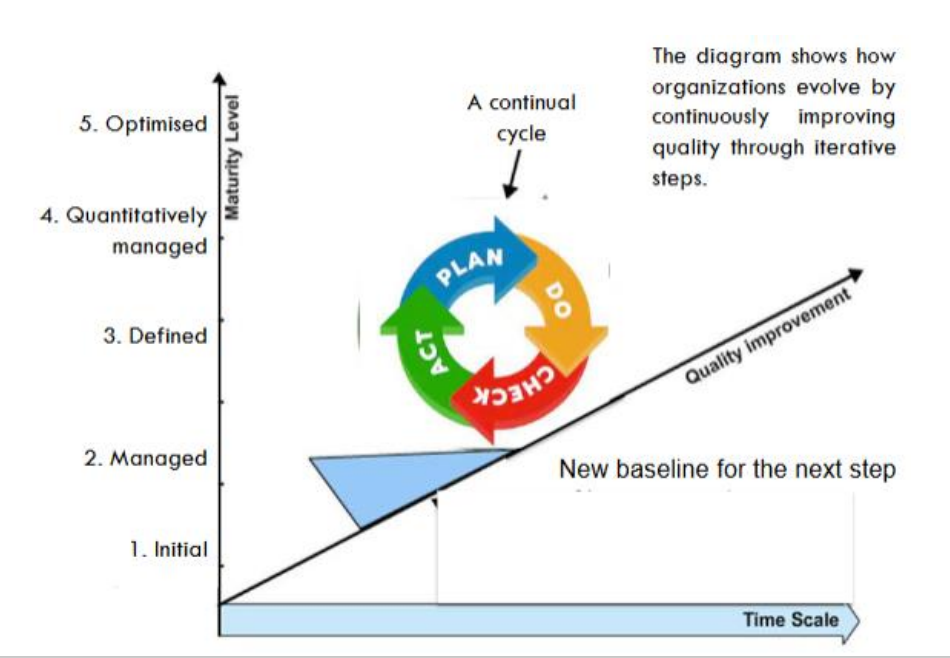
\includegraphics[width=0.8\linewidth]{figures/Week 8/Deming CMMI.png}
\end{figure}

The Deming Cycle (PDCA: Plan–Do–Check–Act) provides a foundation for \textbf{continuous improvement}.

CMMI (Capability Maturity Model Integration) provides a \textbf{structured maturity roadmap} for organizations to evolve their processes.

Together:

\begin{itemize}
    \item Deming $\xrightarrow{}$ How to improve continuously.
    \item CMMI $\xrightarrow{}$ Where the organization stands on process maturity and what the next step is.
\end{itemize}

\bigskip

CMMI Maturity levels:

\begin{itemize}
    \item \textbf{Level 1}: Processes are ad hoc, chaotic. No PDCA cycle in place.
    \item \textbf{Level 2}: Basic planning (Plan) and execution (Do) exist at the project level. However, limited measurement (Check) and corrective actions (Act).
    \item \textbf{Level 3}: Processes are standardized and documented across the organization and consistent Plan–Do; some Check–Act to refine processes.
    \item \textbf{Level 4}: Check phase is emphasized → processes are measured and controlled statistically. Decisions are data-driven.
    \item \textbf{Level 5}: Continuous Act phase → proactive improvements and innovations.
\end{itemize}

\subsubsection{Quality Audits}

\indent 

A Quality Audit is a systematic, independent examination to determine whether activities and related results comply with planned arrangements (such as standards, processes, and requirements) and whether these arrangements are effectively implemented and suitable to achieve objectives.

\bigskip

Main objectives:

\begin{itemize}
    \item Verify compliance with standards, processes, and guidelines.
    \item Identify gaps, inefficiencies, or risks in quality practices.
    \item Recommend improvements for continuous quality enhancement.
    \item Build organizational trust and credibility.
\end{itemize}

\bigskip

Types of Quality Audits:

\begin{itemize}
    \item \textbf{Internal Audits (First-party)}: Conducted by the organization itself. Helps ensure compliance with internal standards and identify early issues.
    \item \textbf{External Audits (Second- and Third-party)}: Conducted by external clients, certification bodies, or regulatory agencies. Ensures independent validation of compliance (e.g., ISO 9000 certification audits).
    \item \textbf{Process Audits}: Focus on whether processes are being followed correctly.
    \item \textbf{Product Audits}: Verify that the end product meets quality specifications and requirements.
    \item \textbf{System Audits}: Evaluate the organization’s overall quality management system (QMS)
\end{itemize}

\subsection{Software Testing Fundamentals}

\subsubsection{Software Testing Lifecycle}

\indent 

\noindent\textbf{Software Testing Lifecycle}: A sequence of specific activities conducted during the testing process to ensure that software meets quality standards.

\bigskip  

Just like the Software Development Lifecycle (SDLC), the STLC is a framework, but it focuses exclusively on \textbf{verification and validation of software}.

\bigskip

\noindent Key features:

\begin{itemize}
    \item Parallel activity to SDLC: Testing starts as soon as requirements are available (shift-left testing).
    \item Iterative process: May repeat for each sprint, release, or version.
    \item Ensures quality at every stage, not just at the end.
\end{itemize}

\subsubsection{Testing Phases}

\begin{table}[h]
\centering
\begin{tabular}{|c|l|l}
\cline{1-2}
\textbf{Phase}                                                                   & \multicolumn{1}{c|}{\textbf{Description}}                                                                                                                                                                  &  \\ \cline{1-2}
\textbf{Requirements}                                                            & \begin{tabular}[c]{@{}l@{}}QA team analyzes requirements (functional and non-functional). \\ They will identify testable requirements and involve stakeholders\\  to clarify any ambiguities.\end{tabular} &  \\ \cline{1-2}
\textbf{Planning}                                                                & \begin{tabular}[c]{@{}l@{}}Define scope, objectives, resources, schedule, and responsibilities. \\ Risks are assessed and mitigation strategies developed.\end{tabular}                                    &  \\ \cline{1-2}
\textbf{Development}                                                             & \begin{tabular}[c]{@{}l@{}}Design test cases with detailed input, expected output, and conditions. \\ Create test data and perform peer review of test cases.\end{tabular}                                 &  \\ \cline{1-2}
\textbf{\begin{tabular}[c]{@{}c@{}}Environment\\ setup\end{tabular}}             & \begin{tabular}[c]{@{}l@{}}Prepare hardware, software, network, and tools for testing. \\ Often involves DevOps pipelines or containerized environments \\ (Docker, Kubernetes, etc.).\end{tabular}        &  \\ \cline{1-2}
\textbf{Execution}                                                               & \begin{tabular}[c]{@{}l@{}}Execute test cases manually or using automation and \\ log test results to raise defect/bug reports for failures.\end{tabular}                                                  &  \\ \cline{1-2}
\textbf{\begin{tabular}[c]{@{}c@{}}Defect reporting\\ and tracking\end{tabular}} & \begin{tabular}[c]{@{}l@{}}Log defects in a bug-tracking system. Prioritise defects \\ and work with developers to ensure timely resolution.\end{tabular}                                                  &  \\ \cline{1-2}
\textbf{Test cycle closure}                                                      & \begin{tabular}[c]{@{}l@{}}Evaluate exit criteria \\ (e.g., all planned test cases executed, critical defects closed). \\ Analyse test coverage and prepare a test summary report (TSR).\end{tabular}      &  \\ \cline{1-2}
\end{tabular}
\end{table}

\subsubsection{Test Artifacts}

\indent 

\textbf{Test artifacts} are the \textbf{documents, deliverables, and by-products} produced during the Software Testing Lifecycle (STLC).

They provide evidence of testing activities, support traceability, and help stakeholders assess software quality.

They can be created before, during, or after testing, and serve as a reference for both current and future projects.

\bigskip

\noindent Benefits of test artifacts:

\begin{itemize}
    \item Traceability: Connects requirements to tests to ensure nothing is missed.
    \item Accountability: Provides evidence of due diligence and compliance (e.g., ISO, CMMI).
    \item Communication: Helps stakeholders (managers, clients, auditors) understand quality status.
\end{itemize}

\subsubsection{Important Test artifacts}

\indent 

\textbf{Test Plan} is a high-level document that defines the scope, approach, objectives, resources, schedule, and responsibilities of testing activities.

Key components:

\begin{itemize}
    \item Objectives and scope of testing
    \item Features to be tested / not tested
    \item Test environment setup
    \item Roles and responsibilities
    \item Schedule and milestones
    \item Risks and mitigation strategies
    \item Tools to be used
\end{itemize}

\bigskip  

A \textbf{Test Case} is a detailed, step-by-step set of instructions to validate a particular functionality of the software. It describes input, execution conditions, and expected output.

Key elements:

\begin{itemize}
    \item Test Case ID
    \item Preconditions (setup required)
    \item Test Steps (actions to perform)
    \item Expected Result
    \item Actual Result (during execution)
    \item Status (Pass/Fail)
\end{itemize}

\bigskip

\textbf{Test Data} refers to the \textbf{input values} (valid, invalid, boundary cases) used in test cases to verify expected system behavior. It ensures tests are realistic and cover a wide range of scenarios.

Types of test data:

\begin{itemize}
    \item Valid Data: Correct input values (e.g., correct username \& password).
    \item Invalid Data: Incorrect inputs (e.g., wrong password, empty fields).
    \item Boundary Data: Edge cases (e.g., password length exactly 8 or 20 chars).
    \item Large Volume Data: For performance/load testing.
\end{itemize}

\newpage

\subsection{Types of Testing}

\subsubsection{Functional vs Non-functional Testing}

\begin{table}[h]
\centering
\begin{tabular}{|c|l|l|}
\hline
\textbf{Aspect}                                                           & \multicolumn{1}{c|}{\textbf{Functional Testing}}                                                                                 & \multicolumn{1}{c|}{\textbf{Non-functional Testing}}                                                                                 \\ \hline
\textbf{Purpose}                                                          & \begin{tabular}[c]{@{}l@{}}Verify that the system\\ behaves according to specified\\ requirements or functionality.\end{tabular} & \begin{tabular}[c]{@{}l@{}}Evaluate how well the system\\ performs under specific conditions\\ (quality attributes).\end{tabular}    \\ \hline
\textbf{Focus}                                                            & \textit{\begin{tabular}[c]{@{}l@{}}What the system does\\ (features, operations,\\ user interactions).\end{tabular}}             & \textit{\begin{tabular}[c]{@{}l@{}}How the system behaves\\ (performance, usability,\\ reliability, security).\end{tabular}}         \\ \hline
\textbf{\begin{tabular}[c]{@{}c@{}}Requirement\\ source\end{tabular}}     & \begin{tabular}[c]{@{}l@{}}Functional requirements\\ (e.g., “User can log in with\\ a username/password”).\end{tabular}          & \begin{tabular}[c]{@{}l@{}}Non-functional requirements\\ (e.g., “System must handle\\ 1000 concurrent users”).\end{tabular}          \\ \hline
\textbf{Test data}                                                        & \begin{tabular}[c]{@{}l@{}}Typically deterministic\\ input/output scenarios.\end{tabular}                                        & \begin{tabular}[c]{@{}l@{}}Often metrics-based:\\ response times, throughput,\\ error rates.\end{tabular}                            \\ \hline
\textbf{\begin{tabular}[c]{@{}c@{}}Automation\\ feasibility\end{tabular}} & \begin{tabular}[c]{@{}l@{}}High\\ (unit and integration tests\\ are commonly automated).\end{tabular}                            & \begin{tabular}[c]{@{}l@{}}Partial\\ (some performance/security\\ tests can be automated;\\ usability is often manual).\end{tabular} \\ \hline
\textbf{\begin{tabular}[c]{@{}c@{}}Examples of\\ tests\end{tabular}}      & \begin{tabular}[c]{@{}l@{}}Unit testing,\\ Integration testing, \\ System testing,\\ User Acceptance Testing, etc.\end{tabular}  & \begin{tabular}[c]{@{}l@{}}Performance testing,\\ Security testing,\\ Usability testing,\\ Compatibility testing, etc.\end{tabular}  \\ \hline
\end{tabular}
\end{table}

\subsubsection{Functional testing - Unit Testing}

\indent 

\begin{figure}[h]
    \centering
    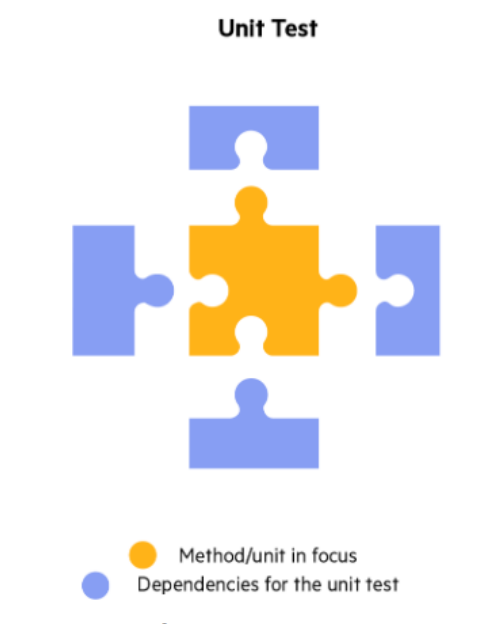
\includegraphics[width=0.3\linewidth]{figures/Week 8/Unit Testing.png}
    \caption{Unit Testing}
\end{figure}

\noindent\textbf{Unit Testing}: Testing the smallest part of an application (a function, method, or class) in isolation.

\noindent\textbf{Goal}: Ensure each unit of code works as expected.

\noindent\textbf{Who does it}: Usually developers.

\subsubsection{Functional testing - Integration Testing}

\indent 

\begin{figure}[h]
    \centering
    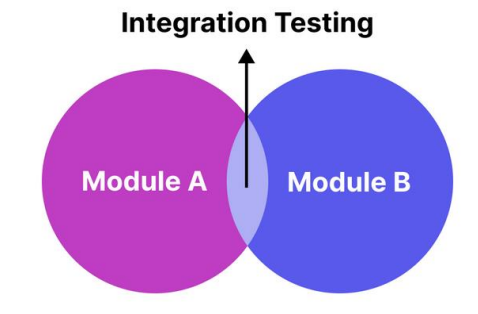
\includegraphics[width=0.5\linewidth]{figures/Week 8/Integration Testing.png}
    \caption{Integration Testing}
\end{figure}

\noindent\textbf{Integration Testing}: Testing interactions between different modules/components.

\noindent\textbf{Goal}: Verify that combined parts work together correctly.

\noindent\textbf{Approaches}:

\begin{itemize}
    \item Big Bang: test everything together at once.
    \item Top-Down: start with higher-level modules, use stubs for lower ones.
    \item Bottom-Up: start with lower modules, use drivers for higher ones.
\end{itemize}

\subsubsection{Functional testing - System Testing}

\indent 

\begin{figure}
    \centering
    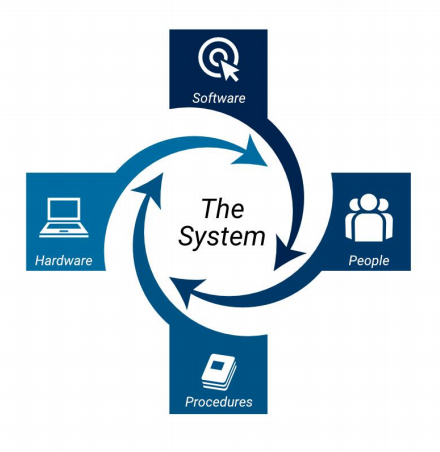
\includegraphics[width=0.3\linewidth]{figures/Week 8/System Testing.png}
    \caption{System Testing}
\end{figure}

\noindent\textbf{System Testing}Testing the complete, integrated system as a whole.
\noindent\textbf{Goal}: Validate that the software meets specified requirements.
\noindent\textbf{Conducted by}: Independent QA/test teams.

\subsubsection{Functional testing - User Acceptance Testing}

\indent 

\noindent\textbf{User Acceptance Testing}: Testing by actual users or clients before release.

\noindent\textbf{Goal}: Ensure the system meets business needs and is ready for production.

\noindent\textbf{Types}:

\begin{itemize}
    \item Alpha Testing: in-house, internal team tests with end-user perspective.
    \item Beta Testing: external users test in real-world environments.
\end{itemize}

\subsubsection{Functional testing - Black Box Testing}

\indent 

\begin{figure}[h]
    \centering
    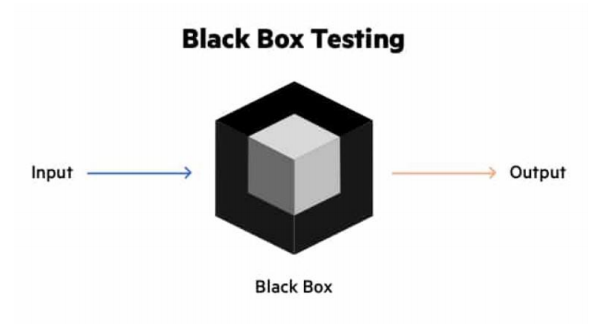
\includegraphics[width=0.3\linewidth]{figures/Week 8/Black Box.png}
    \caption{Black Box Testing}
\end{figure}

\noindent\textbf{Black Box Testing}: Testing without looking at the internal code.

\noindent\textbf{Focus}: Inputs and outputs (functionality).

\noindent\textbf{Techniques}: Boundary value analysis, equivalence partitioning.

\noindent\textbf{Example}: Entering different usernames/passwords to test login functionality

\subsubsection{Functional testing - White Box Testing}

\indent 

\begin{figure}
    \centering
    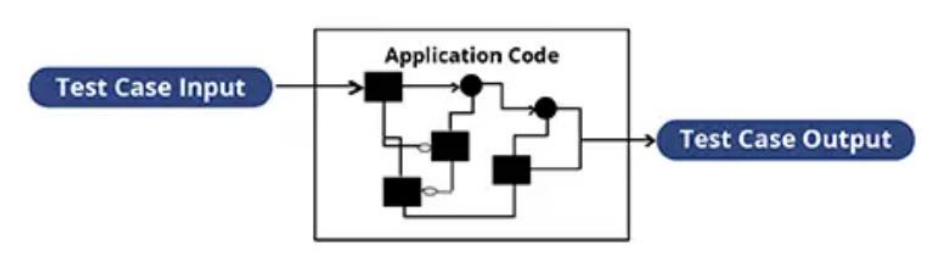
\includegraphics[width=0.3\linewidth]{figures/Week 8/White Box.png}
    \caption{White Box Testing}
\end{figure}

\noindent\textbf{White Box Testing}: Testing the internal logic, paths, and code structure.

\noindent\textbf{Focus}: Code coverage, loops, conditions.

\noindent\textbf{Who does it}: Developers/testers with coding knowledge.

\noindent\textbf{Example}: Writing tests to ensure all branches of an if-else condition execute correctly.

\subsubsection{Non-functional testing - Load Testing}

\indent 

\noindent\textbf{Load Testing}: Checking how the system performs under expected user loads.

\noindent\textbf{Goal}: Measure response time, throughput, and resource usage.

\noindent\textbf{Example}: Simulating 10,000 users logging in to a website simultaneously

\subsubsection{Non-functional testing - Stress Testing}

\indent 

\noindent\textbf{Stress Testing}: Pushing the system beyond normal limits to test breaking points.

\noindent\textbf{Goal}: Identify system stability and recovery after failure.

\noindent\textbf{Example}: Forcing a server to handle 5× expected traffic until it crashes, and observing recovery.

\subsubsection{Non-functional testing - Smoke Testing}

\indent 

\begin{figure}[h]
    \centering
    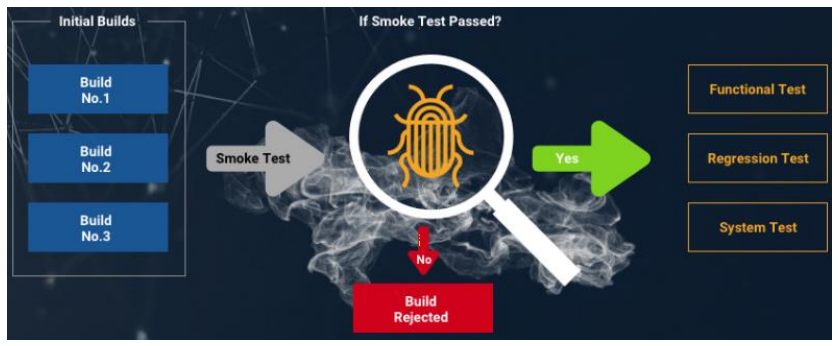
\includegraphics[width=0.8\linewidth]{figures/Week 8/Smoke Testing.png}
    \caption{Smoke Testing}
\end{figure}

\noindent\textbf{Smoke Testing}: A quick check of the basic functionality after a new build or deployment.

\noindent\textbf{Goal}: Ensure the build is stable enough for further testing (“build verification”).

\noindent\textbf{Example}: Verifying that login, navigation, and checkout buttons work after a new release.

\subsubsection{Non-functional testing - A/B Testing}

\indent 

\begin{figure}[h]
    \centering
    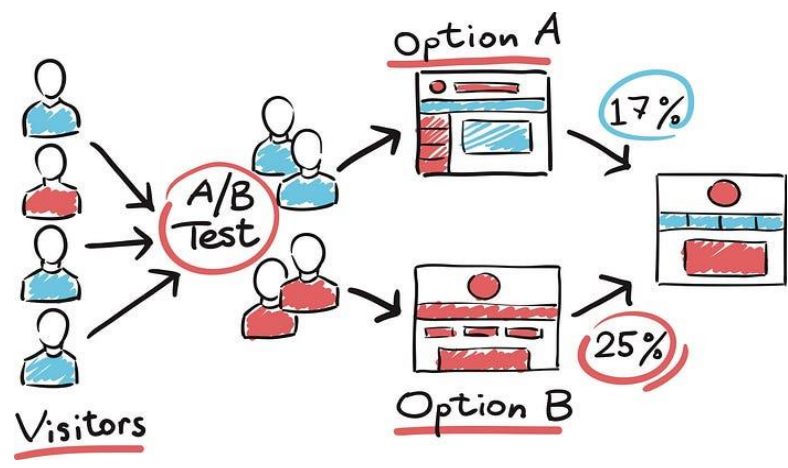
\includegraphics[width=0.8\linewidth]{figures/Week 8/A:B Testing.png}
    \caption{A:B Testing}
\end{figure}

\noindent\textbf{A:B Testing}: Comparing two versions (A and B) to see which performs better with users.

\noindent\textbf{Goal}: Improve usability, conversion, or engagement.

\noindent\textbf{Example}: Version A of a website has a red button, Version B has a blue button $\xrightarrow{}$ measure which drives more clicks.

\subsection{QA in Software Development Methodologies}

\subsubsection{QA in Waterfall}

\indent

QA in Waterfall focuses on \textbf{verification and validation} at \textbf{specific points} in the development lifecycle.

QA activities in each Waterfall Phase

\begin{itemize}
    \item \textbf{Requirements phase}: QA ensures requirements are complete, consistent, and testable.
    \item \textbf{Design phase}: QA verifies system architecture and design documents.
    \item \textbf{Implementation phase}: QA ensures coding standards are followed.
    \item \textbf{Testing phase}: Dedicated QA team executes functional and non-functional testing.
    \item \textbf{Deployment and maintenance phase}: QA ensures release readiness
\end{itemize}

\subsubsection{QA in Agile}

\indent 

QA in Agile is \textbf{integrated throughout the development lifecycle}, not just a separate phase at the end.

QA Activities in Agile:

\begin{itemize}
    \item \textbf{Continuous Requirement Analysis}: QA participates in story refinement and estimation to ensure testable and clear acceptance criteria.
    \item \textbf{Test planning in sprints}: QA plans testing for each sprint (iteration), not for the entire project upfront.
    \item \textbf{Test case design and test data}: QA collaborates closely with developers on test-driven development (TDD) and behavior-driven development (BDD).
    \item \textbf{Continuous testing}: Testing occurs throughout the sprint and defects are identified and fixed immediately, reducing rework costs.
    \item \textbf{Test automation}: Strong emphasis on automation to support fast iteration cycles.
    \item \textbf{Sprint review and retrospective}: QA participates in sprint review to validate delivered features against acceptance criteria.
\end{itemize}

\subsubsection{QA in DevOps}

\indent

QA in DevOps is fully integrated into the software delivery pipeline, emphasizing automation, monitoring, and continuous feedback.

QA activities in DevOps:

\begin{itemize}
    \item QA is \textbf{embedded in CI/CD pipelines}. This allows for early defect detection reduces risks and rework.
    \item DevOps relies heavily on \textbf{test automation} to support rapid releases.
    \item QA begins \textbf{as early as possible} in the development process.
    \item QA monitors \textbf{production environments} for errors, performance issues, and user experience.
    \item QA in DevOps is \textbf{collaborative}, involving developers, testers, operations, and security teams.
\end{itemize}

\subsubsection{Professional Issues in QA}

\indent 

Quality Assurance is not just about processes and testing, it also involves professional and ethical responsibilities. 

Professionals in QA must be aware of \textbf{issues affecting integrity}, \textbf{compliance}, and \textbf{trust} in software systems.

Ethical Responsibilities: QA professionals ensure software is safe, reliable, and meets user requirements.

Compliance and Legal issues: QA professionals must ensure software complies with regulatory and legal standards.

Confidentiality and Data privacy: QA often works with sensitive data (e.g., customer information, financial records).

\subsubsection{Future of QA and Testing}

\indent 

QA is evolving from a \textbf{phase-driven, reactive process to continuous, proactive}, and \textbf{automated quality management}.

Emerging technologies like \textbf{AI, cloud, IoT}, and \textbf{DevOps} are transforming testing practices.

Future QA professionals will need \textbf{technical, analytical}, and \textbf{collaborative skills} to ensure software quality in \textbf{complex, high-speed development environments}.

\subsubsection{How QA Roles Differ Across IT Work Environments}

\begin{table}[h]
\centering
\begin{tabular}{|c|l|l|l|}
\hline
\textbf{Aspect}                                                                 & \multicolumn{1}{c|}{\textbf{Waterfall}}                                                                       & \multicolumn{1}{c|}{\textbf{Agile}}                                                                       & \multicolumn{1}{c|}{\textbf{DevOps}}                                                                                \\ \hline
\textbf{\begin{tabular}[c]{@{}c@{}}When QA\\ happens\end{tabular}}              & At the end of the lifecycle                                                                                   & \begin{tabular}[c]{@{}l@{}}Continuous within\\ sprints\end{tabular}                                       & \begin{tabular}[c]{@{}l@{}}Built into the\\ CI/CD pipeline\end{tabular}                                             \\ \hline
\textbf{\begin{tabular}[c]{@{}c@{}}Your role as \\ a professional\end{tabular}} & \begin{tabular}[c]{@{}l@{}}QA specialist verifies \\ deliverables; strong \\ documentation focus\end{tabular} & \begin{tabular}[c]{@{}l@{}}Developers + QA \\ collaborate closely \\ shared accountability\end{tabular}   & \begin{tabular}[c]{@{}l@{}}Everyone (Dev, QA, \\ Ops, Security) \\ shares responsibility\\ for quality\end{tabular} \\ \hline
\textbf{\begin{tabular}[c]{@{}c@{}}Professional\\ Risk\end{tabular}}            & \begin{tabular}[c]{@{}l@{}}Late defect discovery \\ → high rework cost\end{tabular}                           & \begin{tabular}[c]{@{}l@{}}Missing tests in \\ fast iterations →\\ quality risk\end{tabular}              & \begin{tabular}[c]{@{}l@{}}Over-reliance \\ on automation →\\ oversight risk\end{tabular}                           \\ \hline
\textbf{\begin{tabular}[c]{@{}c@{}}Ethics and\\ Standards\end{tabular}}         & \begin{tabular}[c]{@{}l@{}}Compliance with ISO, \\ CMMI, audit checks\end{tabular}                            & \begin{tabular}[c]{@{}l@{}}Transparency with \\ stakeholders, acceptance \\ criteria clarity\end{tabular} & \begin{tabular}[c]{@{}l@{}}Continuous monitoring,\\ privacy \& security \\ compliance\end{tabular}                  \\ \hline
\end{tabular}
\end{table}

\subsection{Question}

\subsubsection{End of Lecture Questions}

\begin{itemize}
    \item Describe the Deming Cycle (PDCA) and its relevance to QA.
    \item What is CMMI, and how do its maturity levels relate to QA processes?
    \item List and briefly explain the stages of the Software Testing Lifecycle (STLC).
    \item Compare unit testing, integration testing, system testing, and UAT in terms of focus, responsibility, and timing.
    \item Explain how QA differs in Waterfall, Agile, and DevOps methodologies.
    \item How do ISO 9000 and ISO 27001 standards influence QA practices?
\end{itemize}

\subsubsection{Case Study}

\indent 

A bank is developing a new online banking platform that allows customers to log in, transfer funds, pay bills, and view transaction history. During development, several issues were observed:

\begin{itemize}
    \item A critical bug caused login failures for some users.
    \item Transaction processing slowed during peak hours.
    \item Security scans flagged a vulnerability in password storage.
    \item QA documentation was incomplete, leading to missed test cases.
\end{itemize}

\bigskip

\noindent\textbf{Questions}

\begin{itemize}
    \item Describe how traceability between requirements and test cases could prevent missed test cases.
    \item Which type of performance testing would identify the slowdown during peak hours? Explain the difference between load, stress, and soak testing in this context.
    \item Identify professional or ethical issues if the bank released the system with the known login and security issues.
    \item Considering DevOps practices, describe how continuous testing and monitoring could prevent similar issues in production.
\end{itemize}